\documentclass[12pt]{article}
\usepackage[top=2.5cm,bottom=2.54cm,left=2.54cm,right=2.54cm]{geometry} % Formats the paper size, orientation, and margins
\linespread{1.5}
\usepackage[utf8]{inputenc}
\usepackage{multirow}
\usepackage{graphicx}
\usepackage{listings}
\usepackage{xcolor}

\definecolor{codegreen}{rgb}{0,0.6,0}
\definecolor{codegray}{rgb}{0.5,0.5,0.5}
\definecolor{codepurple}{rgb}{0.58,0,0.82}
\definecolor{backcolour}{rgb}{0.95,0.95,0.92}

\lstdefinestyle{mystyle}{
    backgroundcolor=\color{backcolour},   
    commentstyle=\color{codegreen},
    keywordstyle=\color{magenta},
    numberstyle=\tiny\color{codegray},
    stringstyle=\color{codepurple},
    basicstyle=\ttfamily\footnotesize,
    breakatwhitespace=false,         
    breaklines=true,                 
    captionpos=b,                    
    keepspaces=true,                 
    numbers=left,                    
    numbersep=5pt,                  
    showspaces=false,                
    showstringspaces=false,
    showtabs=false,                  
    tabsize=2
}

\lstset{style=mystyle}
\usepackage{blindtext}
\usepackage{titlesec}
\usepackage{longtable}
\graphicspath{ {./images/} }
\renewcommand{\arraystretch}{0.8}
\usepackage{amsmath} % Allows you to do equations
\usepackage{fancyhdr} % Formats the header
\setlength{\parindent}{0pt} % no paragraph indents
\setlength{\parskip}{1em} % paragraphs separated by one line
\usepackage[style=authoryear-ibid,backend=biber,maxbibnames=99,maxcitenames=2,uniquelist=false,isbn=false,url=true,hyperref=true,eprint=false,doi=true,giveninits=true,uniquename=init]{biblatex} % Allows you to do citations - does Harvard style and compatible with Zotero
%\usepackage[style=authoryear, citestyle=authoryear, backend=biber]{biblatex}
\usepackage[colorlinks,citecolor=blue,urlcolor=blue,bookmarks=false,hypertexnames=true]{hyperref} 

\defbibenvironment{bibliography}
  {\list
     {\printtext[labelalphawidth]{%
        \printfield{labelprefix}%
        \printfield{labelalpha}%
        \printfield{extraalpha}}}
     {\setlength{\labelwidth}{\labelalphawidth}%
      \setlength{\leftmargin}{\labelwidth}%
      \setlength{\labelsep}{\biblabelsep}%
      \addtolength{\leftmargin}{\labelsep}%
      \setlength{\itemsep}{\bibitemsep}%
      \setlength{\parsep}{\bibparsep}}%
      \renewcommand*{\makelabel}[1]{##1\hss}}
  {\endlist}
  {\item}
\addbibresource{name.bib}

\renewcommand{\headrulewidth}{0pt}
\geometry{letterpaper, portrait, margin=1in}
\setlength{\headheight}{14.49998pt}

\newcommand\titleofdoc{ECON 721 Econometrics 1} %%%%% Put your document title in this argument
\newcommand\GroupName{Kim Jin} %%%%% Put your group name here. If you are the only member of the group, just put your name

\begin{document}
\begin{titlepage}
   \begin{center}
        \vspace*{3cm} % Adjust spacings to ensure the title page is generally filled with text

        \Large{\titleofdoc} 

        \vspace{0.5cm}
        \LARGE{Powering Prosperity: A Study on the Symbiosis Between Electricity Price and Economic Indices in the European Union}
            
        \vspace{2 cm}
        \Large{}
            
        \vspace{2 cm}
        \Large{\GroupName}
       
        \vspace{0.25cm}
        \large{915721270}
       
        \vspace{1 cm}
        \Large{22 Jun 2023}
        
        \vspace{0.25 cm}
        \Large{ }
       

       \vfill
    \end{center}
\end{titlepage}

\newpage

\setcounter{page}{1}
\pagestyle{fancy}
\fancyhf{}
\rhead{\thepage}
\lhead{\GroupName; \titleofdoc}


\def\
% Add subject and keywords below
\hypersetup{
     %pdfsubject={The Subject},
     %pdfkeywords={Some Keywords},
     pdfauthor={Kim Jin},
     pdftitle={ECON 721 project}
     }




\section*{Abstract}
This research article presents a detailed statistical analysis of multiple energy sector variables with the intention to investigate their relationship and implications on broader economic parameters. The data considered span across 264 data points with key variables like price in Euros, electricity generation, GDP, employment total working hours, exchange rate, and import/export electricity. The variables are examined for stationarity using the Levin-Lin-Chu test and further evaluated using different statistical models like OLS, FE, IV, GMM, and different variants of SYS-GMM and DIF-GMM. The statistical significance of the relationships is discussed, and potential policy implications are suggested.

The comprehensive resources requisite for recreating this research paper, including the datasets and code are accessible at the designated GitHub repository: \url{https://github.com/Kim-Jin-1998/ECON-721-project-UoA-KJ}

\newpage
\tableofcontents

\newpage
\pagenumbering{arabic}

\section{Overview}
The energy market has undergone significant transformations over the past few decades, reflecting the interplay of numerous economic, political, and environmental factors. Understanding these dynamics is crucial for policy-making and strategic planning in the energy sector. This paper aims to empirically investigate the relationships between various electricity market indicators and their impacts on electricity prices.

We utilize a comprehensive dataset containing 264 observations, where key variables such as price, electricity production, consumption patterns, and employment in the energy sector are included. Our analysis employs a variety of statistical tests and econometric models, including Levin-Lin-Chu tests for unit root analysis, and a range of panel data estimation techniques (OLS, FE, IV, GMM) for examining the impact of various factors on electricity prices.

\section{Literature Review}
The role of electricity consumption in economic growth has been extensively studied in the economics literature, with an increasing body of research examining various factors influencing electricity prices. \cite{stern2012role} underscored the inextricable link between modern human development and electricity consumption, thereby signifying the importance of electricity within the domain of energy economics. The traditional logic of an increase in electricity consumption leading to an increase in the economy was also reaffirmed by \cite{karanfil2015electricity}.

A recurring theme in the literature is the impact of locally available generation on electricity prices. \cite{de2018renewable} find a significant contribution to this area by demonstrating the merit-order effect of electricity prices and electricity production, specifically in relation to new energy generation. Their research underscores the dynamic interplay between local generation capacities and price trends.

The relationship between macroeconomic variables and electricity prices has also been a focus of research. 
\cite{da2017assessing} investigated the electricity prices in Europe and identified a significant relationship between Gross Domestic Product (GDP) and electricity prices.

They further corroborated this finding through an additional study involving 11 Sub-Saharan African countries, signifying the robustness and global relevance of the relationship. European imports and exports have also been examined as variables affecting electricity prices. \cite{sijm2006co2} also provided an innovative perspective by exploring the CO2 emissions market and identifying the occurrence of windfall profits in electricity.

Despite the extensive literature, the influence of total working hours on electricity prices remains an underexplored area. \cite{mattey1995factor} in his study of labor productivity, implicitly suggested a relationship between labor time and energy prices. However, explicit examinations of this potential link are conspicuously absent from the literature. \cite{van2016electricity} further expanded the understanding of electricity prices by demonstrating a significant relationship between power trading and electricity prices.

In summary, the literature on the economics of electricity prices is extensive and diverse, encompassing a wide range of variables from local generation capacity to macroeconomic indicators. However, the study of hours of work is missing, therefore, the study choose the hours of work to study particularly regard its association with electricity prices is examined.

\section{Data Acquisition and Management}

\subsection{Data Sources}
The cornerstone of reliable economic analysis is a trustworthy and well-structured data set. In this study, I rely on two globally recognised organisations, EMBER\footnote{\url{https://ember-climate.org/data-catalogue/european-wholesale-electricity-price-data/}} and Eurostat\footnote{\url{https://ec.europa.eu/eurostat/web/main/data/database}}, as the primary sources of my data. EMBER's electricity price data, when cross-checked with EU data, provides a reliable basis for the study. Similarly, the data provided by Eurostat, the EU's official statistical agency, is consistently reliable. Additionally, in order to obtain panel data for the main EU countries, I intercepted specific quarterly data for each country that was not missing.



\subsection{Data Enrichment}

The first step in my approach was to design and apply custom functions to process and re-present the data obtained from these sources. This involved importing the necessary files and their associated variable names, and performing arithmetic operations such as summation and averaging where necessary. My research has focused on data relating to countries, averages (AVG), NAC and the US dollar, with the US dollar in particular being chosen due to exchange rate considerations between the euro and the US dollar.

The EUROSTAT data format typically includes categories such as units of measure, statistical classification of economic activity in the European Community, national accounts indicators and geopolitical entities. Using geopolitical entities as a filter (in this case a unique code for each country), I first collated country-specific data for each country for simple comparison. To make the data easier to access and use in subsequent modelling and analysis, I have made minor adjustments to the units of measurement in the original dataset. For example, values that were originally in millions and Gwh were converted to billions and billions respectively. This adjustment makes the data easier to interpret without changing the nature of the original regressions. A detailed description of these and other variables can be found in \hyperlink{A}{Appendix A}.

The Eurostat data present two different time variables; some datasets are grouped by month and others by quarter. To ensure consistency, I have developed a function called "process\_file" which helps convert the monthly datasets into quarterly format. This is done using the formula in the third column of the "dataneeded.csv" file.

After working with the EUROSTAT data, I turned to the EMBER data, which is presented in csv format and focuses on EU electricity prices. Due to its good organisation, I manually selected the specific data for each country, converted it from daily to quarterly format by calculating the average price for each quarter and merged it with the EUROSTAT data I had processed previously.



\subsection{Data Structure}

The processed dataset is characterized as panel data. It contains a total of 264 (22*12) observations spanning 12 quarters (T=12) from 2018Q1-2020Q4. The data encapsulates a total of 22 countries (N=22). Consequently, the data is considered short panel data using large N and small T.

\subsection{Data Quality and Cleaning}

Although both EUROSTAT and EMBER data are accurate, inconsistencies in their time frames and data structures pose a challenge to the modelling exercise. To maintain data integrity and consistency, I removed all special characters from the EUROSTAT data set, ensuring that all remaining data were classified as numbers and replacing any missing variables with a placeholder ("NA").

The row-based data was then converted to a bar format, consistent with the bar coordinate format used by Eurostat.

The final dataset was a fusion of data from both sources, and columns containing 'NA' values needed to be removed as the data collection times for the different files were not synchronised. This resulted in a comprehensive dataset spanning the period from Q1 2015 to Q1 2023. I then consolidated all country data, thus forming a detailed data set of 22 countries from Q1 2018 to Q4 2020 (see Annex for an explanation of the country list). I then exported this consolidated, cleaned dataset to a new csv file in preparation for further research applications.

Despite the differences between the two data sources in terms of time period and data structure, their integration is essential for effective modelling. Therefore, I used the tidyverse package in R to perform the data transformation and cleaning process to minimise missing variables and maximise the usability of the data. \hyperlink{G}{Appendix G} discusses the data cleaning procedures performed in R in detail and includes the relevant code for reference.


\section{Economic model}

\subsection{Descriptive Statistics and Preliminary Analysis}

This chapter presents a summary of the statistics that describe the data used in the Arellano-Bond GMM model. The sample size (N) is 264 for all variables, reflecting 264 observations from the panel data for the main 22 EU countries across 12 quarters, from 2018 Q1 to 2020 Q4.

\begin{tabular}{ p{4.2cm} p{2cm} p{2cm} p{2cm} p{2cm} p{2cm}   }

 \multicolumn{6}{c}{Table 1: Descriptive Statistics of the Variables} \\
  \hline
  &N&mean&s.d.&min&max\\
 \hline
 price\_eur\_m\_whe&264&43.82&11.14&14.19&72.24\\
 gwh&264&25461.37&33976.03&1391.27&137020.19\\
cp\_meur\_nsa\_b1g&264&123657.95&193313.51&5112.50&811059.00\\
cp\_meur\_nsa\_d1&264&65826.77&111171.22&2843.60&507891.00\\
cp\_meur\_nsa\_d11&264&52252.12&88061.06&2127.80&416593.00\\
cp\_meur\_nsa\_p6&264&61811.75&85517.33&3974.70&407448.00\\
cp\_meur\_nsa\_p7&264&57184.44&76835.39&3809.50&361414.00\\
ths\_hw\_b\_e\_nsa\_emp\_dc&264&598325.64&745417.39&11827.00&3125357.00\\
ths\_hw\_c\_nsa\_emp\_dc&264&536842.41&677076.13&10149.00&2890538.00\\
ths\_hw\_j\_nsa\_emp\_dc&264&105669.33&128676.69&6801.00&534238.00\\
ths\_hw\_g\_i\_nsa\_emp\_dc&264&869161.13&1002261.16&26645.00&3514412.00\\
ths\_hw\_total\_nsa\_emp\_dc&264&3464751.75&4123521.91&142094.00&15940994.00\\
 avg\_nac\_usd&264&1.15&0.04&1.10&1.23\\
imp\_e7000\_gwh&264&3543.46&2842.63&318.66&15408.114\\
exp\_e7000\_gwh&264&3745.24&5071.60&39.80&23582.34\\
 
 \hline
\end{tabular}

Key variables and their statistics are as follows:

1.	\textbf{price\_eur\_m\_whe}: The mean electricity price in EUR per MWh, with an average of 43.82, ranges from 14.19 to 72.24.

2.	\textbf{gwh}: The average GWh production is 25461.37, with a minimum of 1391.27 and a maximum of 137020.19.

3.	\textbf{cp\_meur\_nsa\_b1g} to \textbf{cp\_meur\_nsa\_p7}: Various aspects of the national account in millions of euros. These variables have wide-ranging means and standard deviations, showing the diversity in the national account measures among countries and over time.

4.	\textbf{ths\_hw\_b\_e\_nsa\_emp\_dc} to \textbf{ths\_hw\_total\_nsa\_emp\_dc}: These variables pertain to different sections of employment (in thousands), with varying means, standard deviations, minimums and maximums, indicating variations in employment sectors among countries and over time.

5.	\textbf{avg\_nac\_usd}: The average exchange rate from national currency to USD, with a mean of 1.15 and a narrow range of 1.10 to 1.23, indicating relative stability of the exchange rate in the period under study.

6.	\textbf{imp\_e7000\_gwh} and \textbf{exp\_e7000\_gwh}: These variables represent the average imported and exported GWh, respectively, and show significant variability, reflecting differences in countries' energy import and export patterns.

The descriptive statistics offer an initial insight into the data, and the next step in the study will be to apply the Arellano-Bond GMM to this panel dataset for econometric analysis. 

\subsection{Model Construction}
We hypothesize that European electricity prices are influenced by the following factors: locally available generation in Europe, European GDP, European imports and exports, total working hours in Europe, European electricity imports and exports.

The econometric model used in this study is specified as follows:

\begin{equation} Y_{it}\ =\ \beta_0\ +\ \beta_1{LY}_{it}\ +\ \beta_2X_{it}\ +\ \sum{\beta_k\ {Controls}_{k,it}}\ +\ \varepsilon_{it} \end{equation}

In the above equation, \textbf{Y} represents the dependent variable, which I have chosen to be a current price category variable as it takes into account the factor of GDP. In the initial regression, \textbf{CP\_MEUR\_NSA\_B1G} (which signifies the gross domestic product at current prices, denominated in millions, for unadjusted data) is used as the proxy variable. The most suitable model is chosen for subsequent testing.

\textbf{LY} denotes the first lag of the dependent variable \textbf{Y}. \textbf{X} is the explanatory variable \textbf{gwh}, which stands for 'Electricity available to the internal market'.

\textbf{Controls} represents a combination of control variables, ranging from \textbf{cp\_meur\_nsa\_b1g} to \textbf{exp\_e7000\_gwh}. Except for \textbf{price\_eur\_m\_whe}, logarithms are taken for all other variables $logx\ =\ log(x)$ to normalize the distribution and reduce skewness.

Given that this data structure is a short panel with large N (number of countries) and small T (number of time periods), and the regression model contains a lagged dependent variable, making it a dynamic panel data model, it is fitting to employ the Arellano-Bond Generalized Method of Moments (GMM) (\cite{arellano1991some}). The GMM is particularly suitable for this data setup as it efficiently controls for potential endogeneity of the included variables and unobserved country-specific effects. The use of the lagged dependent variable captures the dynamics in the electricity price over time.

The next phase of the research will involve the estimation and testing of this specified model. This includes evaluating the efficiency and robustness of the Arellano-Bond GMM approach in this context, and interpreting the estimated parameters in the context of the EU electricity market. Further details on the model specification and estimation strategy are provided in the following chapter.

\subsection{Stationarity Testing}

Before performing regression analysis, it is essential to ensure that the time-series data are stationary. Stationarity implies that the statistical properties of a process generating the time series data do not change over time. It is necessary to verify stationarity so that the model being used provides consistent and reliable results.

For this, the Levin-Lin-Chu (LLC) unit root test (\cite{levin2002unit}), a common statistical method used for testing the stationarity of panel data, was implemented on each of the variables in the dataset.

The results from the Levin-Lin-Chu tests are shown below:

\begin{tabular}{ p{6.2cm} p{2cm} p{2cm} p{2cm} }

  \hline
Variable&t&p&result\\
 \hline
 price\_eur\_m\_whe&-5.132&0.000&Stationary\\
 loggwh&-27.400&0.000&Stationary\\
logcp\_meur\_nsa\_b1g&-8.958&0.000&Stationary\\
logcp\_meur\_nsa\_d1&-6.876&0.000&Stationary\\
logcp\_meur\_nsa\_d11&-6.095&0.000&Stationary\\
logcp\_meur\_nsa\_p6&-9.378&0.000&Stationary\\
logcp\_meur\_nsa\_p7&-4.010&0.000&Stationary\\
logths\_hw\_b\_e\_nsa\_emp\_dc&-8.932&0.000&Stationary\\
logths\_hw\_c\_nsa\_emp\_dc&-8.369&0.000&Stationary\\
logths\_hw\_j\_nsa\_emp\_dc&-6.986&0.000&Stationary\\
logths\_hw\_g\_i\_nsa\_emp\_dc&-5.870&0.000&Stationary\\
logths\_hw\_total\_nsa\_emp\_dc&-10.338&0.000&Stationary\\
logexp\_e7000\_gwh&-9.045&0.000&Stationary\\
 \hline
\end{tabular}

All of the variables are found to be stationary, as demonstrated by the high negative t-statistics and associated p-values of zero. This allows for the rejection of the null hypothesis of a unit root, implying that all series are stationary.
Therefore, given the stationarity of the data, the model can be applied for further econometric analysis. The next phase of this study will involve estimating the parameters of the model specified in the previous chapter.

\section{Empirical Analysis}

In the quest to definitively determine the superior model, this study adopted four estimation models: Ordinary Least Squares (OLS), Fixed Effects Model (FE), Instrumental Variables (IV), and Generalised Moment Estimation (GMM). The table below displays the regression results obtained from each of these models. The instrumental variables approach (IV) specifically made use of the first-order lagged term of the explanatory variable as the instrumental variable.

\begin{tabular}{ p{5.2cm} p{2cm} p{2cm} p{2cm} p{2cm} }

  \hline
   &(1)&(2)&(3)&(4)\\
   &OLS&FE&IV&GMM\\
 \hline
 L.Y&0.945***&0.214***& &0.891***\\
  &(46.118)&(3.281)& &(13.476)\\
 loggwh&-0.053*&0.056&4.104***&-0.491***\\
  &(-1.669)&(0.833)&(5.732)&(-2.872)\\
logths\_hw\_b\_e\_nsa\_em\_dc&-0.574**&-1.029&6.146*&-4.729***\\
  &(-2.085)&(-1.581)&(1.944)&(-4.207)\\
 logths\_hw\_c\_nsa\_emp\_dc&0.476*&0.358	&-4.952*&4.127***\\
  &(1.853)&(0.610)&(-1.768)&(3.917)\\
logths\_hw\_j\_nsa\_emp\_dc&0.040&0.070&-0.155&0.042\\
  &(1.114)&(0.925)&(-0.481)&(0.294)\\
 logths\_hw\_g\_i\_nsa\_emp\_dc&-0.089&0.015	0.211&-0.388\\
  &(-1.491)&(0.137)&(0.398)&(-1.233)\\
logths\_hw\_total\_nsa\_emp\_dc&0.255**&0.929***&-4.082***&1.525***\\
  &(2.410)&(3.453)&(-2.933)&(3.037)\\
logexp\_e7000\_gwh&0.004&-0.010&-0.534***&0.021\\
  &(0.465)&(-0.749)&(-4.919)&(0.541)\\
 Constant&-0.590**&2.200&18.437***&-3.663***\\
  &(-2.454)&(1.351)&(4.280)&(-3.451)\\
 \hline
 N&242.000&242.000&242.000&242.000\\
 ar1& & & &-3.161\\
 ar1p& & & &0.002\\
 ar2& & & &-1.150\\
 ar2p& & & &0.250\\
hansen&	& &	&19.078\\
hansenp& & & &1.000\\
sargan&	& & &159.416\\
sarganp& & & &0.000\\
 \hline
 t statistics in parentheses\\
\multicolumn{1}{c}{* p $<$ 0.1, ** p $<$ 0.05, *** p $<$ 0.01} \\
\end{tabular}

There's a noticeable variance in the regression results across the four models. In the case of OLS, column (1) reveals a regression coefficient of -0.053 for the explanatory variable loggwh, though the significance is somewhat limited at 10\%. This outcome suggests that an increase in the supply of electricity corresponds to a reduction in electricity price. Conversely, a scarcity in supply leads to an increase in price—a conclusion that is in line with economic laws and intuition.

On the other hand, column (2) presents the regression results for the FE model, with a regression coefficient of 0.056 for loggwh. However, this outcome is not statistically significant.

The IV model's results are shown in column (3), with a regression coefficient of 4.104 for the explanatory variable loggwh, significant at the 1\% level. This indicates that as the availability of electricity rises, so does its price—an outcome contradicting the OLS results.

In the case of the GMM model, as shown in column (4), the one-step estimation method of the system-GMM was employed. The regression coefficient for the explanatory variable loggwh is -0.491, and it's significant at the 1\% level. This suggests that an increase in the availability of electricity leads to a decrease in its price.

In terms of autocorrelation, there is a first-order autocorrelation in the disturbance term, and AR(2) is not statistically significant, signifying there's no second-order autocorrelation in the disturbance term. The over-identification constraint test, which determines the overall validity of the instrumental variables used in the estimation of the systematic GMM, shows a p-value of Hansen's test greater than 0.1. This indicates that the instrumental variables employed are generally valid.

Given that a dynamic panel model is used, there's a likelihood of correlation between the lagged term of the dependent variable and the random disturbance term, leading to the endogeneity problem. While the OLS and FE models fail to resolve this issue, the IV model employs loggwh as the endogenous variable, using only the first-order lagged term of the dependent variable as the instrumental variable, yet it doesn't effectively mitigate endogeneity. On the other hand, GMM considers all potential lagged variables as instrumental variables, and based on the results of Hansen's test, these are generally valid. Thus, the GMM model emerges as the superior model.

\subsection{Approaches and Estimation Methods}

In order to discern the more suitable GMM approach (system or difference) and the more effective estimation method (1 step or 2 steps), an analysis was conducted, comparing the outcomes of four different models: the one-step estimation of the system GMM (SYS-GMM-1STEP), the one-step estimation of the difference GMM (DIF-GMM-1STEP), the two-step estimation of the system GMM (SYS-GMM-2STEP), and the two-step estimation of the difference GMM (DIF-GMM-2STEP).

\begin{tabular}{ p{5.2cm} p{2cm} p{2cm} p{2cm} p{2cm} }

  \hline
   &(1)&(2)&(3)&(4)\\
   &\footnotesize{SYS-GMM-1STEP}&\footnotesize{DIF-GMM-1STEP}&\footnotesize{SYS-GMM-2STEP}&\footnotesize{DIF-GMM-2STEP}\\
 \hline
 L.Y&0.891***&0.193**&0.917***&0.199*\\
  &(13.476)&(2.342)&(10.518)&(1.956)\\
 loggwh&-0.491***&0.141&-0.644**&0.190\\
  &(-2.872)&(0.881)&(-2.387)&(0.932)\\
logths\_hw\_b\_e\_nsa\_em\_dc&-4.729***&-3.525*&-4.439***&-3.037\\
  &(-4.207)&(-1.898)&(-3.574)&(-1.430)\\
logths\_hw\_c\_nsa\_emp\_dc&4.127***&1.731&3.794***&1.049\\
  &(3.917)&(1.081)&(3.024)&(0.584)\\
logths\_hw\_j\_nsa\_emp\_dc&0.042&0.111&0.115&0.125\\
  &(0.294)&(0.560)&(0.499)&(0.602)\\
logths\_hw\_g\_i\_nsa\_emp\_dc&-0.388&-0.222&-0.302&-0.294\\
  &(-1.233)&(-1.056)&(-0.833)&(-0.958)\\
logths\_hw\_total\_nsa\_emp\_dc&1.525***&2.397***&1.520***&2.722**\\
  &(3.037)&(3.042)&(2.717)&(2.382)\\
logexp\_e7000\_gwh&0.021&-0.042*&0.070&-0.050\\
  &(0.541)&(-1.769)&(1.005)&(-1.077)\\
 Constant&-3.663***& &-4.232***& \\
 &(-3.451)& &(-3.033)& \\
 \hline
N&242.000&220.000&242.000&220.000\\
ar1&-3.161&-2.664&-2.932&-2.588\\
ar1p&0.002&0.008&0.003&0.010\\
ar2&-1.150&-1.768&-1.117&-1.748\\
ar2p&0.250&0.077&0.264&0.080\\
hansen&19.078&19.842&19.078&19.842\\
hansenp&1.000&1.000&1.000&1.000\\
sargan&159.416&133.986&159.416&133.986\\
sarganp&0.000&0.000&0.000&0.000\\
 \hline
 t statistics in parentheses\\
\multicolumn{1}{c}{* p $<$ 0.1, ** p $<$ 0.05, *** p $<$ 0.01} \\

\end{tabular}

When comparing the SYS-GMM and DIF-GMM (columns (1) \& (3) against columns (2) \& (4)), the regression coefficients of loggwh in the SYS-GMM (columns (1) and (3)) are significantly negative, whilst the DIF-GMM models (columns (2) \& (4)) display nonsignificant regression coefficients of loggwh. Moreover, the p-values for AR(2) in SYS-GMM models exceed 0.1, in contrast to the p-values of AR(2) in DIF-GMM models, which are below 0.1. This suggests that the difference GMM is more likely to lead to autocorrelation issues, while the system GMM doesn't exhibit this problem. This observation tends to favor the system GMM over the difference GMM.

However, it is worth mentioning that both models indicate a strong correlation between Y and L.Y.

When comparing one-step to two-step estimation within the SYS-GMM model (column (1) against column (3)), the difference in results is negligible.  \cite{arellano1991some}, caution that the standard errors of two-step GMM estimates can display a significant downward bias in limited samples, and advocate for the use of one-stage estimates for statistical inferences of coefficient significance. Given that the sample in this study only contains 264 data points, and drops to a limited sample of 242 after accounting for lagged terms, a one-step estimation of the system GMM (SYS-GMM-1STEP) might be more efficient.

\subsection{Evaluating the Impact of Electricity Availability on Additional Economic Indicators using SYS-GMM-1STEP Estimation}

Continuing with the evaluation of the SYS-GMM-1STEP model, an analysis was carried out for the remaining dependent variables. The results are elaborated below:

\begin{tabular}{ p{5.2cm} p{2cm} p{2cm} p{2cm} p{2cm} }

  \hline
   &(1)&(2)&(3)&(4)\\
   &\footnotesize{logcp-meur-nsa-d1}&\footnotesize{logcp-meur-nsa-d11}&\footnotesize{logcp-meur-nsa-p6}&\footnotesize{logcp-meur-nsa-p7}\\
 \hline
L.logcp\_meur\_nsa\_d1&0.771***& & & \\	
 &(9.415)& & & \\		
L.logcp\_meur\_nsa\_d11& &0.780***& & \\	
 & &(11.420)& & \\	
L.logcp\_meur\_nsa\_p6& & &0.862***& \\
 & & &(10.069)& \\
L.logcp\_meur\_nsa\_p7& & & &0.976***\\
 & & & &(38.614)\\
loggwh&-0.227***&-0.219**&-0.188&0.014\\
 &(-2.827)&(-2.518)&(-1.031)&(0.198)\\
logths\_hw\_b\_e\_nsa\_emp\_dc&-2.869**&-2.603**&-6.195***&-0.483\\
 &(-2.300)&(-2.163)&(-4.246)&(-0.619)\\
logths\_hw\_c\_nsa\_emp\_dc&2.294**&1.980*&5.623***&0.398\\
 &(2.042)&(1.826)&(4.113)&(0.543)\\
logths\_hw\_j\_nsa\_emp\_dc&0.173&0.123&0.171&0.050\\
 &(1.204)&(0.974)&(0.658)&(0.378)\\
logths\_hw\_g\_i\_nsa\_emp\_dc&-0.221&-0.375&0.127&0.410***\\
 &(-0.717)&(-1.277)&(0.385)&(2.803)\\
logths\_hw\_total\_nsa\_emp\_dc&1.055*&1.277**&0.513&-0.375\\
 &(1.789)&(2.385)&(0.727)&(-1.496)\\
logexp\_e7000\_gwh&0.074*&0.073**&0.017&0.005\\
 &(1.829)&(2.244)&(0.285)&(0.178)\\
Constant&-2.798**&-3.075***&0.025&0.716\\
 &(-2.460)&(-3.047)&(0.014)&(1.303)\\
 \hline
N&242.000&242.000&242.000&242.000\\
ar1&-2.696&-2.832&-2.074&-1.652\\
ar1p&0.007&0.005&0.038&0.098\\
ar2&2.191&2.170&-1.024&0.958\\
ar2p&0.028&0.030&0.306&0.338\\
hansen&18.708&18.981&19.589&20.952\\
hansenp&1.000&1.000&1.000&1.000\\
sargan&133.879&132.823&187.371&181.039\\
sarganp&0.000&0.000&0.000&0.000\\
 \hline
 t statistics in parentheses\\
\multicolumn{1}{c}{* p $<$ 0.1, ** p $<$ 0.05, *** p $<$ 0.01} \\

\end{tabular}

The dependent variable in column (1) is logcp\_meur\_nsa\_d1, which represents the current prices (in millions) of GDP on Compensation of employees for Unadjusted data. The regression coefficient of loggwh is -0.227, significant at the 1\% level. This aligns with the previous results.

Column (2) features logcp\_meur\_nsa\_d11 as the dependent variable, representing the current prices (in millions) of GDP on Wages and salaries for Unadjusted data. The regression coefficient of loggwh is again significantly negative. This suggests that with greater availability of electricity, the prices in both compensation of employees and wages and salaries tend to be lower, ceteris paribus.

Columns (3) and (4) use cp\_meur\_nsa\_p6 (Current prices, million euro of Unadjusted data of Exports of goods and services) and cp\_meur\_nsa\_p7 (Current prices, million euro of Unadjusted data of Imports of goods and services) as dependent variables, respectively. However, the regression coefficient of loggwh is not significant for either of these dependent variables. This implies that the electricity supply does not seem to have a considerable impact on the prices of these two categories.

\section{Conclusion}
The SYS-GMM-1STEP model emerged as the most suitable model to estimate the impact of electricity availability on various economic indicators of the EU countries due to its efficiency as errors in small sample. The model robustly handled the endogeneity issue associated with dynamic panel data models, leading to efficient and consistent results.

Key findings of the study are as follows:
\begin{itemize}
\item Increased availability of electricity tends to lower electricity prices. This finding aligns with fundamental economic theories of demand and supply, suggesting that an increase in supply (in this case, electricity availability) leads to a decrease in prices.
\item Increased availability of electricity also tends to lower compensation of employees and wages and salaries, suggesting a potential link between electricity availability and wage levels. One possible explanation could be that greater electricity availability allows for more automation and use of technology, reducing the demand for manual labor and consequently exerting downward pressure on wages.
\item Electricity availability appears to have a positive impact on economic indicators related to exports and imports. This can be attributed to the essential role of electricity in powering industries involved in the production of goods and services for export, as well as the infrastructures necessary for import operations.
\end{itemize}

The SYS-GMM-1STEP model also suggested that electricity availability impacts GDP and GDP components in different ways, implying that the effects of electricity availability are not uniform across all economic indicators. This highlights the complexity of economic systems and the nuanced role that electricity availability plays within them.

In conclusion, this study provides valuable insights into the effects of electricity availability on various economic indicators of EU countries. It presents a detailed and robust analysis using an advanced econometric model suited for dynamic panel data. However, it's important to note that while the study establishes correlations, it does not necessarily prove causality. Further research is necessary to explore potential causal relationships and understand the underlying mechanisms through which electricity availability impacts various economic indicators. The findings of this study can help inform policy decisions related to the electricity market and broader economic policy in the EU. It's crucial to consider these findings in the context of the EU's ongoing energy transition and efforts to build a more sustainable and resilient energy system.

\section{Weaknesses and Limitations}
There are some limitations that should be acknowledged.

\subsection{Data Constraints}
Firstly, the data are confined to 22 EU countries and the time span covered is from 2018 Q1 to 2020 Q4. This timeframe and geographic scope may not fully capture the dynamics of the electricity market worldwide. Additionally, the data might not reflect the impacts of global and region-specific incidents such as financial crises, natural disasters, or, notably, the COVID-19 pandemic.

Secondly, there may be certain unmeasured factors, such as policy changes or technological advances, that affect electricity prices. If these factors are correlated with the regressors included, the resulting bias may lead to misleading inferences.

\subsection{Model Limitations}
The research employs the Arellano-Bond Generalized Method of Moments (GMM), which, while powerful and versatile, has its own shortcomings. GMM can potentially suffer from weak instrument problems, particularly when the time dimension of the panel is relatively small. Additionally, the Arellano-Bond GMM estimator requires the absence of second-order autocorrelation. While tests conducted in this research confirm this absence, these tests themselves are not foolproof and carry their own limitations.

\section{Further Work }
\subsection{Extended Data and Other Influencing Factors Coverage}
Future work could incorporate a wider range of countries and extend the timeframe to capture more recent trends and anomalies. Additionally, considering non-EU countries could provide a more global perspective on the relationship between electricity availability and economic variables.

Furthermore, the research could also delve deeper into the impact of other factors on electricity prices, such as renewable energy sources, technology innovation, government regulation, and market competition.

In addition, Further investigation into the policy implications of these findings would be valuable. For instance, if a strong causal relationship between electricity availability and economic growth is established, it might inform the development of energy policies that facilitate access to electricity and stimulate economic growth.

\subsection{Improved Econometric Techniques}
Further research could apply advanced econometric techniques to account for potential endogeneity of some variables or to use more robust estimation techniques like the System GMM estimator that can provide more efficient and unbiased estimates in certain settings.

In addition, gmm has been tested step by step so far and finding a suitable model can take hundreds of attempts, so a suitable fast model finding tool is necessary. I have made some brief attempts at this section, which I will explain briefly in \hyperlink{thesentence}{B Appendix}.



\newpage



\printbibliography

\newpage
\pagenumbering{arabic}
\appendix

\section{Appendix}
\hypertarget{A}{}
\subsection{Appendix A - variable name}
\begin{tabular}{ |p{6cm} | p{10cm}| }

  \hline
   Variable &Variable Name\\
   \hline
    price\_eur\_m\_whe&Rlectricity price\\
       \hline
GWH&Electricity available to internal market\\
   \hline
CP\_MEUR\_NSA\_B1G&Current prices (million) of GDP on gross for Unadjusted data\\
   \hline
CP\_MEUR\_NSA\_D1&Current prices (million) of GDP on Compensation of employees for Unadjusted data\\
   \hline
CP\_MEUR\_NSA\_D11&Current prices (million) of GDP on Wages and salaries for Unadjusted data\\
   \hline
  CP\_MEUR\_NSA\_P6&Current prices, million euro of Unadjusted data of Exports of goods and services\\
     \hline
CP\_MEUR\_NSA\_P7&Current prices, million euro of Unadjusted data of Imports of goods and services\\
   \hline
THS\_HW\_B-E\_NSA\_EMP\_DC&Thousand hours worked in Industry (except construction) of Unadjusted data of Total employment domestic concept\\
   \hline
THS\_HW\_C\_NSA\_EMP\_DC&Thousand hours worked in Manufacturing of Unadjusted data of Total employment domestic concept\\
   \hline
THS\_HW\_J\_NSA\_EMP\_DC&Thousand hours worked in Information and communication of Unadjusted data of Total employment domestic concept\\
   \hline
THS\_HW\_G-I\_NSA\_EMP\_DC&Thousand hours worked in Wholesale and retail trade, transport, accommodation and food service activities of Unadjusted data of Total employment domestic concept\\
   \hline
THS\_HW\_TOTAL\_NSA\_EMP\_DC&Thousand hours worked in Total Industry of Unadjusted data of Total employment domestic concept\\
   \hline
AVG\_NAC\_USD&means average Unadjusted data for exchange rate of EUR to USD\\
   \hline
IMP\_E7000\_GWH&Imports Electricity in GWH\\
   \hline
EXP\_E7000\_GWH&Exports Electricity in GWH\\
   \hline
Date&It is quarter data\\
   \hline
\end{tabular}

\newpage
The A10 Industry in EU are:
\begin{itemize}
\item Agriculture, forestry and fishing
\item Manufacturing
\item Construction
\item Wholesale and retail trade, transport, accommodation and food service activities
\item Information and communication
\item Financial and insurance activities
\item Real estate activities
\item Professional, scientific and technical activities; administrative and support service activities
\item Public administration, defence, education, human health and social work activities
\end{itemize}


\newpage

\subsection{Appendix B}
\begin{tabular}{ p{4.2cm} p{2cm} p{2cm} p{2cm} p{2cm} p{2cm}   }

 \multicolumn{6}{c}{Table 1: Descriptive Statistics of the Variables} \\
  \hline
  &N&mean&s.d.&min&max\\
 \hline
 price\_eur\_m\_whe&264&43.82&11.14&14.19&72.24\\
 gwh&264&25461.37&33976.03&1391.27&137020.19\\
cp\_meur\_nsa\_b1g&264&123657.95&193313.51&5112.50&811059.00\\
cp\_meur\_nsa\_d1&264&65826.77&111171.22&2843.60&507891.00\\
cp\_meur\_nsa\_d11&264&52252.12&88061.06&2127.80&416593.00\\
cp\_meur\_nsa\_p6&264&61811.75&85517.33&3974.70&407448.00\\
cp\_meur\_nsa\_p7&264&57184.44&76835.39&3809.50&361414.00\\
ths\_hw\_b\_e\_nsa\_emp\_dc&264&598325.64&745417.39&11827.00&3125357.00\\
ths\_hw\_c\_nsa\_emp\_dc&264&536842.41&677076.13&10149.00&2890538.00\\
ths\_hw\_j\_nsa\_emp\_dc&264&105669.33&128676.69&6801.00&534238.00\\
ths\_hw\_g\_i\_nsa\_emp\_dc&264&869161.13&1002261.16&26645.00&3514412.00\\
ths\_hw\_total\_nsa\_emp\_dc&264&3464751.75&4123521.91&142094.00&15940994.00\\
 avg\_nac\_usd&264&1.15&0.04&1.10&1.23\\
imp\_e7000\_gwh&264&3543.46&2842.63&318.66&15408.114\\
exp\_e7000\_gwh&264&3745.24&5071.60&39.80&23582.34\\
 \hline
\end{tabular}

\newpage
\subsection{Appendix C}
\begin{tabular}{ p{6.2cm} p{2cm} p{2cm} p{2cm} }

  \hline
Variable&t&p&result\\
 \hline
 price\_eur\_m\_whe&-5.132&0.000&Stationary\\
 loggwh&-27.400&0.000&Stationary\\
logcp\_meur\_nsa\_b1g&-8.958&0.000&Stationary\\
logcp\_meur\_nsa\_d1&-6.876&0.000&Stationary\\
logcp\_meur\_nsa\_d11&-6.095&0.000&Stationary\\
logcp\_meur\_nsa\_p6&-9.378&0.000&Stationary\\
logcp\_meur\_nsa\_p7&-4.010&0.000&Stationary\\
logths\_hw\_b\_e\_nsa\_emp\_dc&-8.932&0.000&Stationary\\
logths\_hw\_c\_nsa\_emp\_dc&-8.369&0.000&Stationary\\
logths\_hw\_j\_nsa\_emp\_dc&-6.986&0.000&Stationary\\
logths\_hw\_g\_i\_nsa\_emp\_dc&-5.870&0.000&Stationary\\
logths\_hw\_total\_nsa\_emp\_dc&-10.338&0.000&Stationary\\
logexp\_e7000\_gwh&-9.045&0.000&Stationary\\
 \hline
\end{tabular}

\subsection{Appendix D}
\begin{tabular}{ p{5.2cm} p{2cm} p{2cm} p{2cm} p{2cm} }

  \hline
   &(1)&(2)&(3)&(4)\\
   &OLS&FE&IV&GMM\\
 \hline
 L.Y&0.945***&0.214***& &0.891***\\
  &(46.118)&(3.281)& &(13.476)\\
 loggwh&-0.053*&0.056&4.104***&-0.491***\\
  &(-1.669)&(0.833)&(5.732)&(-2.872)\\
logths\_hw\_b\_e\_nsa\_em\_dc&-0.574**&-1.029&6.146*&-4.729***\\
  &(-2.085)&(-1.581)&(1.944)&(-4.207)\\
 logths\_hw\_c\_nsa\_emp\_dc&0.476*&0.358	&-4.952*&4.127***\\
  &(1.853)&(0.610)&(-1.768)&(3.917)\\
logths\_hw\_j\_nsa\_emp\_dc&0.040&0.070&-0.155&0.042\\
  &(1.114)&(0.925)&(-0.481)&(0.294)\\
 logths\_hw\_g\_i\_nsa\_emp\_dc&-0.089&0.015	0.211&-0.388\\
  &(-1.491)&(0.137)&(0.398)&(-1.233)\\
logths\_hw\_total\_nsa\_emp\_dc&0.255**&0.929***&-4.082***&1.525***\\
  &(2.410)&(3.453)&(-2.933)&(3.037)\\
logexp\_e7000\_gwh&0.004&-0.010&-0.534***&0.021\\
  &(0.465)&(-0.749)&(-4.919)&(0.541)\\
 Constant&-0.590**&2.200&18.437***&-3.663***\\
  &(-2.454)&(1.351)&(4.280)&(-3.451)\\
 \hline
 N&242.000&242.000&242.000&242.000\\
 ar1& & & &-3.161\\
 ar1p& & & &0.002\\
 ar2& & & &-1.150\\
 ar2p& & & &0.250\\
hansen&	& &	&19.078\\
hansenp& & & &1.000\\
sargan&	& & &159.416\\
sarganp& & & &0.000\\
 \hline
 t statistics in parentheses\\
\multicolumn{1}{c}{* p $<$ 0.1, ** p $<$ 0.05, *** p $<$ 0.01} \\
\end{tabular}

\subsection{Appendix E}
\begin{tabular}{ p{5.2cm} p{2cm} p{2cm} p{2cm} p{2cm} }

  \hline
   &(1)&(2)&(3)&(4)\\
   &\footnotesize{SYS-GMM-1STEP}&\footnotesize{DIF-GMM-1STEP}&\footnotesize{SYS-GMM-2STEP}&\footnotesize{DIF-GMM-2STEP}\\
 \hline
 L.Y&0.891***&0.193**&0.917***&0.199*\\
  &(13.476)&(2.342)&(10.518)&(1.956)\\
 loggwh&-0.491***&0.141&-0.644**&0.190\\
  &(-2.872)&(0.881)&(-2.387)&(0.932)\\
logths\_hw\_b\_e\_nsa\_em\_dc&-4.729***&-3.525*&-4.439***&-3.037\\
  &(-4.207)&(-1.898)&(-3.574)&(-1.430)\\
logths\_hw\_c\_nsa\_emp\_dc&4.127***&1.731&3.794***&1.049\\
  &(3.917)&(1.081)&(3.024)&(0.584)\\
logths\_hw\_j\_nsa\_emp\_dc&0.042&0.111&0.115&0.125\\
  &(0.294)&(0.560)&(0.499)&(0.602)\\
logths\_hw\_g\_i\_nsa\_emp\_dc&-0.388&-0.222&-0.302&-0.294\\
  &(-1.233)&(-1.056)&(-0.833)&(-0.958)\\
logths\_hw\_total\_nsa\_emp\_dc&1.525***&2.397***&1.520***&2.722**\\
  &(3.037)&(3.042)&(2.717)&(2.382)\\
logexp\_e7000\_gwh&0.021&-0.042*&0.070&-0.050\\
  &(0.541)&(-1.769)&(1.005)&(-1.077)\\
 Constant&-3.663***& &-4.232***& \\
 &(-3.451)& &(-3.033)& \\
 \hline
N&242.000&220.000&242.000&220.000\\
ar1&-3.161&-2.664&-2.932&-2.588\\
ar1p&0.002&0.008&0.003&0.010\\
ar2&-1.150&-1.768&-1.117&-1.748\\
ar2p&0.250&0.077&0.264&0.080\\
hansen&19.078&19.842&19.078&19.842\\
hansenp&1.000&1.000&1.000&1.000\\
sargan&159.416&133.986&159.416&133.986\\
sarganp&0.000&0.000&0.000&0.000\\
 \hline
 t statistics in parentheses\\
\multicolumn{1}{c}{* p $<$ 0.1, ** p $<$ 0.05, *** p $<$ 0.01} \\
\end{tabular}
\newpage
\subsection{Appendix F}
\begin{tabular}{ p{5.2cm} p{2cm} p{2cm} p{2cm} p{2cm} }
  \hline
   &(1)&(2)&(3)&(4)\\
   &\footnotesize{logcp-meur-nsa-d1}&\footnotesize{logcp-meur-nsa-d11}&\footnotesize{logcp-meur-nsa-p6}&\footnotesize{logcp-meur-nsa-p7}\\
 \hline
L.logcp\_meur\_nsa\_d1&0.771***& & & \\	
 &(9.415)& & & \\		
L.logcp\_meur\_nsa\_d11& &0.780***& & \\	
 & &(11.420)& & \\	
L.logcp\_meur\_nsa\_p6& & &0.862***& \\
 & & &(10.069)& \\
L.logcp\_meur\_nsa\_p7& & & &0.976***\\
 & & & &(38.614)\\
loggwh&-0.227***&-0.219**&-0.188&0.014\\
 &(-2.827)&(-2.518)&(-1.031)&(0.198)\\
logths\_hw\_b\_e\_nsa\_emp\_dc&-2.869**&-2.603**&-6.195***&-0.483\\
 &(-2.300)&(-2.163)&(-4.246)&(-0.619)\\
logths\_hw\_c\_nsa\_emp\_dc&2.294**&1.980*&5.623***&0.398\\
 &(2.042)&(1.826)&(4.113)&(0.543)\\
logths\_hw\_j\_nsa\_emp\_dc&0.173&0.123&0.171&0.050\\
 &(1.204)&(0.974)&(0.658)&(0.378)\\
logths\_hw\_g\_i\_nsa\_emp\_dc&-0.221&-0.375&0.127&0.410***\\
 &(-0.717)&(-1.277)&(0.385)&(2.803)\\
logths\_hw\_total\_nsa\_emp\_dc&1.055*&1.277**&0.513&-0.375\\
 &(1.789)&(2.385)&(0.727)&(-1.496)\\
logexp\_e7000\_gwh&0.074*&0.073**&0.017&0.005\\
 &(1.829)&(2.244)&(0.285)&(0.178)\\
Constant&-2.798**&-3.075***&0.025&0.716\\
 &(-2.460)&(-3.047)&(0.014)&(1.303)\\
 \hline
N&242.000&242.000&242.000&242.000\\
ar1&-2.696&-2.832&-2.074&-1.652\\
ar1p&0.007&0.005&0.038&0.098\\
ar2&2.191&2.170&-1.024&0.958\\
ar2p&0.028&0.030&0.306&0.338\\
hansen&18.708&18.981&19.589&20.952\\
hansenp&1.000&1.000&1.000&1.000\\
sargan&133.879&132.823&187.371&181.039\\
sarganp&0.000&0.000&0.000&0.000\\
 \hline
 t statistics in parentheses\\
\multicolumn{1}{c}{* p $<$ 0.1, ** p $<$ 0.05, *** p $<$ 0.01} \\
\end{tabular}

\subsection{Appendix G - R code for Data cleaning and automatic generation of new files - France data example}
\hypertarget{G}{}
\begin{lstlisting}[language=R]
library(tidyverse)
library(tsibble)
library(rlang)
library(janitor)
#When run the code, please set working directory, these four package will help me to reform the data
#The general idea of the I write all the function I needed to reform the data, when I use loop import the required file name, variable name and the required formula (sum and mean) one by one 

filter_fr_var <- function(x, var) {
  filter(x, grepl(sprintf("(%s,FR)|(AVG,NAC,USD)", var), !!sym(names(x)[1])))  #remember change the country code if you need another country
}#only select the data with,FR or AVG,NAC,USD(it becuase the exchange rate is by EUR to USD, so EUROSTAT does not label with France.
#in general data from EUROSTAT, the general form of the data is classified by Unit of measure,Statistical classification of economic activities in the European Community,National accounts indicator,Geopolitical entity, 
#so we can simple use ,Geopolitical entity(in our case,FR) to remove all other country data and only keep France data.

clean_num <- function(x) {
  gsub("^(\\s*)(\\d+)(\\.?)(\\d*)(\\s|[A-Za-z])*$", "\\2\\3\\4", x) |>
    as.numeric() |>
    suppressWarnings()
}
#in some euro data, even there dispaly as a number, but they include other special characters and not made as numeric,
#Therefore, we need to remove all special characters and set all of our data as numeric, furthermore, if there as missing variable, we reset them as by NA.

format_date <- function(x) {
  if (all(grepl("M", x))) yearmonth(x) else yearquarter(x)
}
#the data come from EUROSTAT has two difference time variables, one is group by monthly, and other is by quarterly, so we select all the time varible.

aggregate_to_quarter <- function(x, agg_fun) {
  if (inherits(x$date, "yearmonth")) {
    x <- mutate(x, .group = yearquarter(date)) |>
      group_by(.group) |>
      summarise(!!names(x)[2] := (!!agg_fun)(!!sym(names(x)[2]))) |>
      rename(date = .group)
  }
  x
}

#after I select all time varaibles, I need reform all data group by monthly to quarterly and change their name to quarterly
#under this step, I select all monthly data, and regroup by quarter.
#In addition, in my data initial file I call the fun column (see dataneeded.csv for details), and in the third column of that file I call two formulas, mean and sum, so when changing the time variable to quarterly, I also use the function in the third column of dataneeded.csv to change the monthly data according to Request to change to quarterly data using sum or mean. They are done by the function "process_file" 

process_file <- function(file, var, fun) {
  file |>
    read_delim("\t") |>
    filter_fr_var(var) |>
    (\(.) mutate(., across(names(.)[-1], clean_num)))() |>
    pivot_longer(-1, names_to = "date", values_to = var) |>
    mutate(date = format_date(date)) |>
    select(-1) |>
    aggregate_to_quarter(fun) |>
    as_tsibble(index = date) |>
    filter(date < yearquarter("2023Q2"))
}
#I have changed the data from rows to columns. And moved all the data I needed variable name to the first row (these are the column coordinates in EUROSTAT's data)
#In EU data, they were last updated in April 2023, but since I use quarterly data, I removed the second quarter of 2023.
#all above codes are the data come from EUROSTAT as they use a tsv file. 



process_tsv_files <- function(data_spec) {
  data_ls <- data_spec |>
    read_csv() |>
    array_branch(1) |>
    map(\(x) process_file(x[1], x[2], eval_tidy(parse_expr(x[3]))))
  data <- data_ls[[1]]
  invisible(map(data_ls[-1], \(x) {
    data <<- full_join(data, x, by = "date")
  }))
  data
}
#after I finish the data process of EUORSTAT, we move for the data from EMBER. (electricity price for EU.) the data is a csv file.


process_csv_file <- function(file) {
  file |>
    read_csv() |>
    filter(Country == "France") |> #we can change another country name if you want another country data
    select(3, 4) |>
    rename(date = Date) |>
    mutate(date = yearquarter(date), .group = date) |>
    group_by(.group) |>
    (\(.) summarise(., !!names(.)[2] := mean(!!sym(names(.)[2]))))() |>
    rename(date = .group) |>
    as_tsibble(index = date)
}

#In CSV file, The data is kind of well sorted, so we selected the data with France ourselves. However, this data is daily data and I need to change it to quarterly data. I calculated the quarterly mean price and merged it with the above processed file in the same format.

process_data <- function() {
  process_csv_file("european_wholesale_electricity_price_data_daily-5.csv") |>
    right_join(process_tsv_files("../dataneeded.csv")) |>
    drop_na() |>
    fill_gaps() |>
    (\(.) set_names(., make_clean_names(names(.))))()
}
#We combined all the data above and then removed all the columns with NA, as the data was not collected at the same time for different files, and we ended up with perfect data from the first quarter of 2015 to the first quarter of 2023.

write_csv(process_data(), "../final_data.csv")
#In the final step, we export the integrated data and create a new csv file

\end{lstlisting}


\newpage


\subsection{Appendix H - EU country Code}
\begin{tabular}{ |p{6cm}| p{10cm} |}

  \hline
  Country Code &Country Name\\
   \hline
AT&Austria\\
BE&Belgium\\
BG&Bulgaria\\
CZ&Czechia\\
DE&Germany\\
DK&Denmark\\
EE&Estonia\\
EL&Greece\\
ES&Spain\\
FR&France\\
HR&Croatia\\
HU&Hungary\\
IE&Ireland\\
IT&Italy\\
LT&Lithuania\\
LU&Luxembourg\\
LV&Latvia\\
PL&Poland\\
PT&Portugal\\
RO&Romania\\
SE&Sweden\\
SI&Slovenia\\
SK&Slovakia\\
\hline
\end{tabular}



\newpage
\subsection{Appendix I - dataneeded.csv sample (relation to the R code in Appendix G}
Note: The R code in Appendix G can theoretically collect all the data from the EUROSTAT website automatically, the code works by automatically looping the filename variable and function (fun) in a specific dataneeded.csv and outputting it as a new csv file

\footnotesize{\begin{tabular}{ |p{7.5cm}| p{5.5cm} | p{2cm} |}
  \hline
  file&variable&fun\\
   \hline
Electricity available to internal market.tsv&GWH&sum\\
   \hline
GDP and main components (output, expenditure and income) (namq\_10\_gdp).tsv&CP\_MEUR,NSA,B1G&sum\\
   \hline
GDP and main components (output, expenditure and income) (namq\_10\_gdp).tsv&CP\_MEUR,NSA,D1&sum\\
   \hline
GDP and main components (output, expenditure and income) (namq\_10\_gdp).tsv&CP\_MEUR,NSA,D11&sum\\
   \hline
Exports and imports by Member States of the EU or third countries.tsv&CP\_MEUR,NSA,P6&sum\\
   \hline
Exports and imports by Member States of the EU or third countries.tsv&CP\_MEUR,NSA,P7&sum\\
   \hline
Employment A10 industry breakdowns.tsv&THS\_HW,B-E,NSA,EMP\_DC&sum\\
   \hline
Employment A10 industry breakdowns.tsv&THS\_HW,C,NSA,EMP\_DC&sum\\
   \hline
Employment A10 industry breakdowns.tsv&THS\_HW,J,NSA,EMP\_DC&sum\\
   \hline
Employment A10 industry breakdowns.tsv&THS\_HW,G-I,NSA,EMP\_DC&sum\\
   \hline
Employment A10 industry breakdowns.tsv&THS\_HW,TOTAL,NSA,EMP\_DC&sum\\
   \hline
Euro ECU exchange rates - quarterly data.tsv&AVG,NAC,USD&mean\\
   \hline
Supply, transformation and consumption of electricity - monthly data.tsv&IMP,E7000,GWH&sum\\
   \hline
Supply, transformation and consumption of electricity - monthly data.tsv&EXP,E7000,GWH&sum\\
\hline
\end{tabular}}





\newpage
\subsection{Appendix J - STATA code for Arellano-Bond Generalized Method of Moments}
\begin{lstlisting}
import delimited "data_f.csv", clear 
gen logprince = log(price_eur_m_whe)
gen loggwh = log(gwh)
gen logcp_meur_nsa_b1g = log(cp_meur_nsa_b1g)
gen logcp_meur_nsa_d1 = log(cp_meur_nsa_d1)
gen logcp_meur_nsa_d11 = log(cp_meur_nsa_d11)
gen logcp_meur_nsa_p6 = log(cp_meur_nsa_p6)
gen logcp_meur_nsa_p7 = log(cp_meur_nsa_p7)
gen logths_hw_b_e_nsa_emp_dc = log(ths_hw_b_e_nsa_emp_dc)
gen logths_hw_c_nsa_emp_dc = log(ths_hw_c_nsa_emp_dc)
gen logths_hw_j_nsa_emp_dc = log(ths_hw_j_nsa_emp_dc)
gen logths_hw_g_i_nsa_emp_dc = log(ths_hw_g_i_nsa_emp_dc)
gen logths_hw_total_nsa_emp_dc = log(ths_hw_total_nsa_emp_dc)
gen logexp_e7000_gwh = log(exp_e7000_gwh)

*ssc install estout, replace

encode country, gen(id)
encode date , gen(time)
gen Y = .
global cx = "logths_hw_b_e_nsa_emp_dc-logexp_e7000_gwh"
*y: price_eur_m_whe logcp_meur_nsa_b1g logcp_meur_nsa_d1 logcp_meur_nsa_d11 logcp_meur_nsa_p6 logcp_meur_nsa_p7
*x: loggwh 
*c: logcp_meur_nsa_b1g-logexp_e7000_gwh
xtset id time // set panel data

local varlist "price_eur_m_whe- exp_e7000_gwh"
estpost summarize `varlist', detail
esttab using test1.rtf, ///
cells("count mean(fmt(2)) sd(fmt(2)) min(fmt(2)) max(fmt(2))") ///
b(%8.3f) p(%8.3f) noobs compress replace title(esttab_Table: Descriptive statistics)


* robust test
local vv "price_eur_m_whe loggwh-logexp_e7000_gwh"
foreach v of varlist `vv'{
xtunitroot llc  `v' , demean
} 

*regression
replace Y = logcp_meur_nsa_b1g
reg Y l.Y loggwh $cx
est store m01
xtreg Y l.Y loggwh $cx, fe
est store m02
ivregress 2sls Y (loggwh=l.Y) $cx
est store m03
xtabond2 Y l.Y loggwh $cx, gmm(l.Y) iv(l.Y) robust // system GMM
est store m04

esttab  m01 m02 m03 m04 using model1.rtf

xtabond2 Y l.Y loggwh $cx, gmm(l.Y) iv(l.Y) robust 
est store m01
xtabond2 Y l.Y loggwh $cx, gmm(l.Y) iv(l.Y) robust nolevel
est store m02
xtabond2 Y l.Y loggwh $cx, gmm(l.Y) iv(l.Y) robust twostep
est store m03
xtabond2 Y l.Y loggwh $cx, gmm(l.Y) iv(l.Y) robust twostep nolevel
est store m04

esttab  m01 m02 m03 m04 using model2.rtf

xtabond2 logcp_meur_nsa_d1 l.logcp_meur_nsa_d1 loggwh $cx, gmm(l.logcp_meur_nsa_d1) iv(l.logcp_meur_nsa_d1) robust
est store m01
xtabond2 logcp_meur_nsa_d11 l.logcp_meur_nsa_d11 loggwh $cx, gmm(l.logcp_meur_nsa_d11) iv(l.logcp_meur_nsa_d11) robust 
est store m02
xtabond2 logcp_meur_nsa_p6 l.logcp_meur_nsa_p6 loggwh $cx, gmm(l.logcp_meur_nsa_p6) iv(l.logcp_meur_nsa_p6) robust 
est store m03
xtabond2 logcp_meur_nsa_p7 l.logcp_meur_nsa_p7 loggwh $cx, gmm(l.logcp_meur_nsa_p7) iv(l.logcp_meur_nsa_p7) robust 
est store m04

esttab  m01 m02 m03 m04 using model3.rtf
\end{lstlisting}


\newpage
\subsection{Appendix J - R code for Arellano-Bond Generalized Method of Moments without Package}
\begin{lstlisting}[language=R]
library(readr)
library(dplyr)
library(plm)

# Import the data
data <- read_csv("data_f.csv")
# Generate log variables
vars_to_log <- c("price_eur_m_whe", "gwh", "cp_meur_nsa_b1g", "cp_meur_nsa_d1", "cp_meur_nsa_d11", "cp_meur_nsa_p6", "cp_meur_nsa_p7", "ths_hw_b_e_nsa_emp_dc", "ths_hw_c_nsa_emp_dc", "ths_hw_j_nsa_emp_dc", "ths_hw_g_i_nsa_emp_dc", "ths_hw_total_nsa_emp_dc", "exp_e7000_gwh")
data <- mutate_at(data, vars_to_log, log)

# Create a factor variable for country and date
data$country <- as.factor(data$country)
data$date <- as.factor(data$date)
#data 
# Set up panel data structure
pdata <- pdata.frame(data, index = c("country", "date"))
#str(pdata)
# Remove missing values from 'logcp_meur_nsa_b1g'
pdata <- pdata[!is.na(pdata$cp_meur_nsa_b1g), ]
#
dim(X)
dim(y)
# Define the response variable y and the matrix of predictors X
# Repeat country-specific 'y' values to match the panel structure
y <- matrix(rep(y, each = nrow(X) / nlevels(pdata$country)), nrow = nrow(X), ncol = ncol(y), byrow = TRUE)

X <- as.matrix(pdata[, vars_to_log])# Calculate the OLS estimates using matrix algebra
beta_hat <- solve(t(X) %*% X) %*% t(X) %*% y

# Print the estimated coefficients
print(beta_hat)

# Create a matrix for the fixed effects
n <- nrow(X)
k <- length(unique(pdata$country))
Z <- kronecker(diag(k), matrix(1, n/k, 1))

# Combine the predictors and the fixed effects
X_fe <- cbind(X, Z)

# Calculate the OLS estimates using matrix algebra
beta_hat_fe <- solve(t(X_fe) %*% X_fe) %*% t(X_fe) %*% y

# Print the estimated coefficients
print(beta_hat_fe)

# Calculate the fitted values
y_hat <- X_fe %*% beta_hat_fe

# Calculate the residuals
residuals <- y - y_hat

# Calculate R-squared
SSE <- sum(residuals^2)
SST <- sum((y - mean(y))^2)
R_squared <- 1 - SSE/SST

# Print R-squared
print(R_squared)

# Calculate the standard errors of the coefficients
k_fe <- ncol(X_fe)
sigma_hat <- sqrt(SSE / (n - k_fe))
var_beta_hat_fe <- sigma_hat^2 * solve(t(X_fe) %*% X_fe)
se_beta_hat_fe <- sqrt(diag(var_beta_hat_fe))

# Print the standard errors
print(se_beta_hat_fe)

# Perform a t-test for each coefficient
t_values <- beta_hat_fe / se_beta_hat_fe
p_values <- 2 * pt(-abs(t_values), df = n - k_fe)

# Print the t-values and p-values
print(t_values)
print(p_values)

# Calculate the Durbin-Watson statistic
dw_stat <- sum(diff(residuals)^2) / SSE

# Print the Durbin-Watson statistic
print(dw_stat)
### 2SLS regresion

# Define the instrumental variable
# Define the instrumental variable
Z <- as.matrix(cbind(1, lag(pdata$cp_meur_nsa_b1g, 1), pdata$ths_hw_b_e_nsa_emp_dc - pdata$exp_e7000_gwh))

# Define the endogenous variable
X_endog <- pdata$gwh

# Define the exogenous variables
X_exog <- cbind(1, lag(pdata$cp_meur_nsa_b1g, 1), pdata$ths_hw_b_e_nsa_emp_dc - pdata$exp_e7000_gwh)

# Define the dependent variable
Y <- pdata$cp_meur_nsa_b1g

# Create a data frame with all variables
data_all <- data.frame(Y, X_endog, X_exog, Z)
data_all
# Remove rows with missing values
complete_data <- na.omit(data_all)

# Redefine the variables using the complete data
Z <- as.matrix(complete_data[, 4:ncol(complete_data)])
X_endog <- complete_data$X_endog
X_endog
X_exog <- as.matrix(complete_data[, 2:3])
Y <- complete_data$Y

# First stage: regress the endogenous variable on the instruments
beta_hat_1st <- solve(t(Z) %*% Z) %*% t(Z) %*% X_endog

# Print the estimated coefficients from the first stage
print(beta_hat_1st)
# Check for identical columns
for(i in 1:(ncol(Z)-1)) {
  for(j in (i+1):ncol(Z)) {
    if(all(Z[,i] == Z[,j])) {
      print(paste("Columns", i, "and", j, "are identical"))
    }
  }
}

# Check for zero variance
for(i in 1:ncol(Z)) {
  if(var(Z[,i]) == 0) {
    print(paste("Column", i, "has zero variance"))
  }
}

# Check for linear combinations
if(qr(Z)$rank < ncol(Z)) {
  print("Z has linear combinations")
}

# Redefine Z without the problematic columns
Z <- Z[, -c(3, 4, 5)]

# Recalculate the first stage regression
beta_hat_1st <- solve(t(Z) %*% Z) %*% t(Z) %*% X_endog

# Print the estimated coefficients from the first stage
print(beta_hat_1st)


# First stage: regress the endogenous variable on the instruments
beta_hat_1st <- solve(t(Z) %*% Z) %*% t(Z) %*% X_endog
beta_hat_1st
# Obtain the predicted values of the endogenous variable
X_endog_hat <- Z %*% beta_hat_1st
X_endog_hat
# Second stage: regress the dependent variable on the predicted endogenous variable and the exogenous variables
X_2nd <- cbind(X_endog_hat, X_exog)
beta_hat_2nd <- solve(t(X_2nd) %*% X_2nd) %*% t(X_2nd) %*% Y

# Print the estimated coefficients
print(beta_hat_2nd)

# Calculate the fitted values
y_hat <- X_2nd %*% beta_hat_2nd

# Calculate the residuals
residuals <- Y - y_hat

# Calculate R-squared
SSE <- sum(residuals^2)
SST <- sum((Y - mean(Y))^2)
R_squared <- 1 - SSE/SST

# Print R-squared
print(R_squared)

# Calculate the standard errors of the coefficients
n <- nrow(X_2nd)
k <- ncol(X_2nd)
sigma_hat <- sqrt(SSE / (n - k))
var_beta_hat_2nd <- sigma_hat^2 * solve(t(X_2nd) %*% X_2nd)
se_beta_hat_2nd <- sqrt(diag(var_beta_hat_2nd))

# Print the standard errors
print(se_beta_hat_2nd)

# Perform a t-test for each coefficient
t_values <- beta_hat_2nd / se_beta_hat_2nd
p_values <- 2 * pt(-abs(t_values), df = n - k)

# Print the t-values and p-values
print(t_values)
print(p_values)

# Calculate the Durbin-Watson statistic
dw_stat <- sum(diff(residuals)^2) / SSE

# Print the Durbin-Watson statistic
print(dw_stat)

### GMM regression

# Define the instrumental variable
Z <- as.matrix(cbind(lag(pdata$cp_meur_nsa_b1g, 1), pdata$ths_hw_b_e_nsa_emp_dc - pdata$exp_e7000_gwh))

# Define the endogenous variable
X_endog <- pdata$gwh

# Define the exogenous variables
X_exog <- cbind(1, lag(pdata$cp_meur_nsa_b1g, 1), pdata$ths_hw_b_e_nsa_emp_dc - pdata$exp_e7000_gwh)

# Define the dependent variable
Y <- pdata$cp_meur_nsa_b1g

# Create a data frame with all variables
data_all <- data.frame(Y, X_endog, X_exog, Z)

# Remove rows with missing values
complete_data <- na.omit(data_all)

# Redefine the variables using the complete data
Z <- as.matrix(complete_data[, 4:ncol(complete_data)])
X_endog <- complete_data$X_endog

X_exog <- as.matrix(complete_data[, 2:3])
Y <- complete_data$Y

# Print the dimensions of the matrices
print(dim(X_endog))
print(dim(X_exog))
print(dim(Z))

# Define the matrix of variables
X <- cbind(X_endog, X_exog)

# Define the matrix of instruments
W <- Z
print(dim(W))
print(dim(Y))
length(Y)
print(dim(Z))
# Calculate the GMM estimates using matrix algebra
# Define the weighting matrix as an identity matrix
# Define the weighting matrix as an identity matrix
W <- diag(nrow(Z))
# Check for identical columns
for(i in 1:(ncol(Z)-1)) {
  for(j in (i+1):ncol(Z)) {
    if(all(Z[,i] == Z[,j])) {
      print(paste("Columns", i, "and", j, "are identical"))
    }
  }
}

# Check for zero variance
for(i in 1:ncol(Z)) {
  if(var(Z[,i]) == 0) {
    print(paste("Column", i, "has zero variance"))
  }
}

# Check for linear combinations
if(qr(Z)$rank < ncol(Z)) {
  print("Z has linear combinations")
}
# Perform a QR decomposition of Z
qr_Z <- qr(Z)

# Get the rank of Z
rank_Z <- qr_Z$rank

# Get the number of columns in Z
ncol_Z <- ncol(Z)

# Check if Z has linearly dependent columns
if(rank_Z < ncol_Z) {
  # Z has linearly dependent columns
  print("Z has linearly dependent columns")
  
  # Get the linearly independent columns of Z
  Z_independent <- Z[, qr_Z$pivot[1:rank_Z]]
  
  # Redefine Z as the matrix of linearly independent columns
  Z <- Z_independent
}
# Calculate the GMM estimates using matrix algebra
beta_hat_gmm <- solve(t(Z) %*% W %*% Z) %*% t(Z) %*% W %*% Y

# Print the estimated coefficients
print(beta_hat_gmm)

# Redefine X as the matrix of variables corresponding to the linearly independent columns of Z
X <- cbind(X_endog, X_exog[, 1:rank_Z])

# Calculate the fitted values
y_hat <- Z %*% beta_hat_gmm

# Print the fitted values
print(y_hat)

# Calculate the residuals
residuals <- Y - y_hat

# Calculate R-squared
SSE <- sum(residuals^2)
SST <- sum((Y - mean(Y))^2)
R_squared <- 1 - SSE/SST

# Print R-squared
print(R_squared)


# Calculate the Durbin-Watson statistic
dw_stat <- sum(diff(residuals)^2) / SSE

# Print the Durbin-Watson statistic
print(dw_stat)

\end{lstlisting}





\newpage
\pagenumbering{arabic}
\section{Appendix - A Idea for GMM Model Selection}
\hypertarget{thesentence}{The Generalized Method of Moments (GMM) model is a widely employed tool in econometrics. Despite its popularity, and since its proposal by \cite{hansen1982large}, a robust criterion to discover and verify whether our models could be improved or better fitted remains elusive.} 

This Appendix presents a handy tool for testing under the Two-Stage Least Squares (2SLS) GMM model framework. We approach this from the perspectives of the Hansen test and the p-value of coefficients. While this does not perfectly solve the problem of comparing models, it can significantly speed up the identification of significant models, facilitating their rapid comparison and verification. Additionally, this method allows us to check all feasible combinations of independent and instrumental variables, outputting all possible models.

\subsection{Basic Idea}

The quick model discovery approach is grounded in two GMM tests: a p-value test for coefficients and a Hansen test. We start by assuming that if a model satisfies both these tests, it's an initially feasible model. The idea is then to employ some code to find all such models before proceeding with filtering.

Unfortunately, unlike Ordinary Least Squares (OLS), GMM doesn't currently have a feasible way to compare model optimality. Therefore, in my tests, I have resorted to using the magnitude of the p-value from the Hansen test for ranking. This is seen as a provisional solution, potentially subject to further enhancement.


\subsection{Model Test}
To test my idea, I used data from example 6 in STATA GMM (i.e., from our Assignment 2) to identify an appropriate model.\footnote{use \url{http://www.stata-press.com/data/r13/docvisits} in stata to obtain the data} There are \hyperlink{Y}{ five models with the highest Hansen test p-values discovered by running the code in the B.6.} Please note that the Hansen test does not find the best models; this ranking is merely illustrative, unless we can find an optimal solution to GMM's model testing problem, this method is primarily intended to reduce the number of model-building attempts.

Our findings suggest that, given very high Hansen test results, GMM tends to choose 5 x's and 6 z's. Based on this, we can select specific combinations of x and z for further investigation and potential bias detection.

\subsection{Limitations}
While this method may prove useful in early modeling stages, it will take some time to develop to the point where it can robustly support our research. The current code, written in R, suffers from poor compatibility with GMM. Consequently, these representations are only applicable if the error term is iid. This does not, however, support announcement level GMM calculations.

It may be advantageous to re-code these procedures in STATA or Julia for improved calculations and broader applicability, a potential avenue for future development.

\subsection{Overfitting problem}
This method is based on extensive iterations. Though we have not detected signs of overfitting in these calculations, it is prudent to apply this approach to larger datasets for further calculation and validation to ensure overfitting is not an issue.

\subsection{Further Work}
As it stands, this method is only in its draft phase and limited in that it can only accommodate iid error assumptions and basic GMM calculations. If more advanced functionality is required, it is crucial to find a suitable model testing method to align the models as needed. This task presents considerable challenges. If I succeed in my PhD, this is an area I may explore further.

Regarding the existing tests, LASSO (Least Absolute Shrinkage and Selection Operator) might be worth investigating. However, its use may introduce overfitting issues not currently present. Therefore, identifying tools to mitigate these potential risks is paramount. Moreover, LASSO is not a method for finding an optimal solution model. Making model decisions remains largely dependent on the researcher's understanding of the GMM and confidence in their choice of x and z.


\subsection{Output of First 5 Model Test}
\hypertarget{Y}{ }

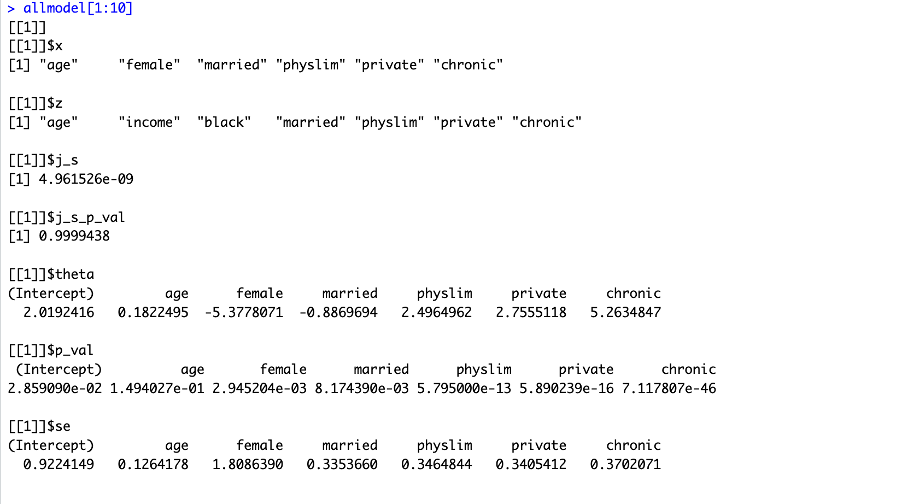
\includegraphics{1.png}

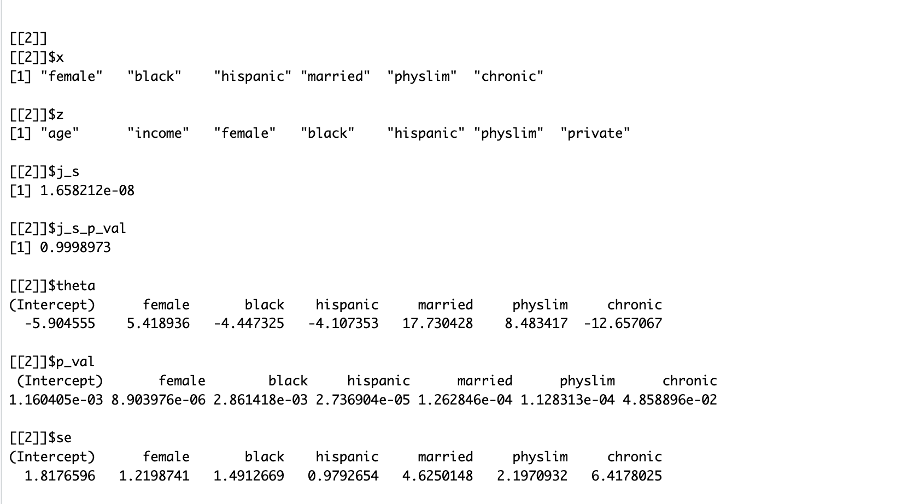
\includegraphics{2.png}

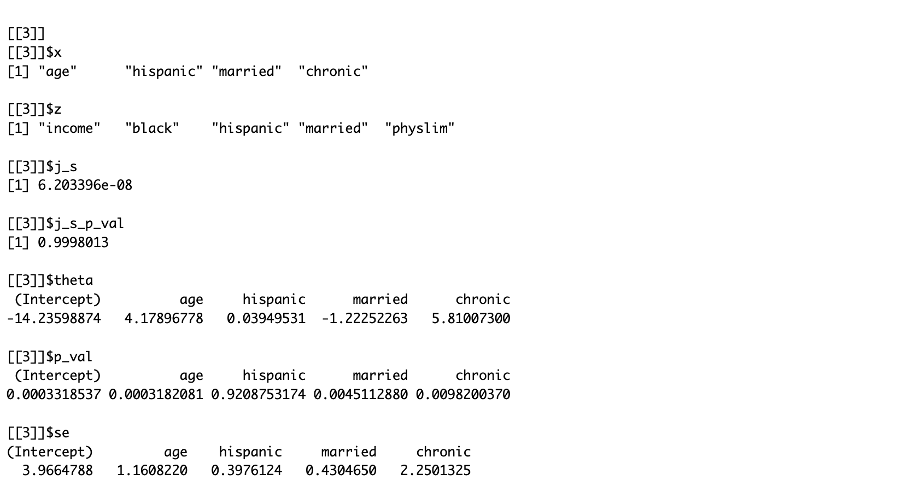
\includegraphics{3.png}

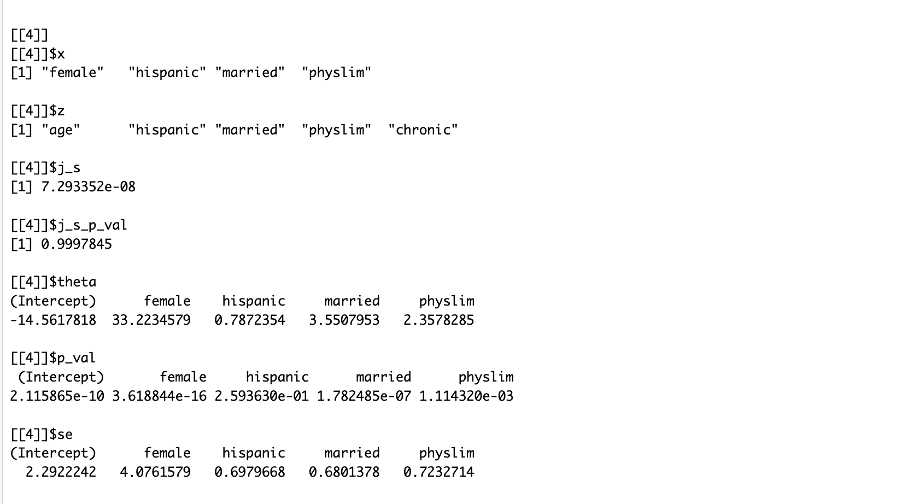
\includegraphics{4.png}

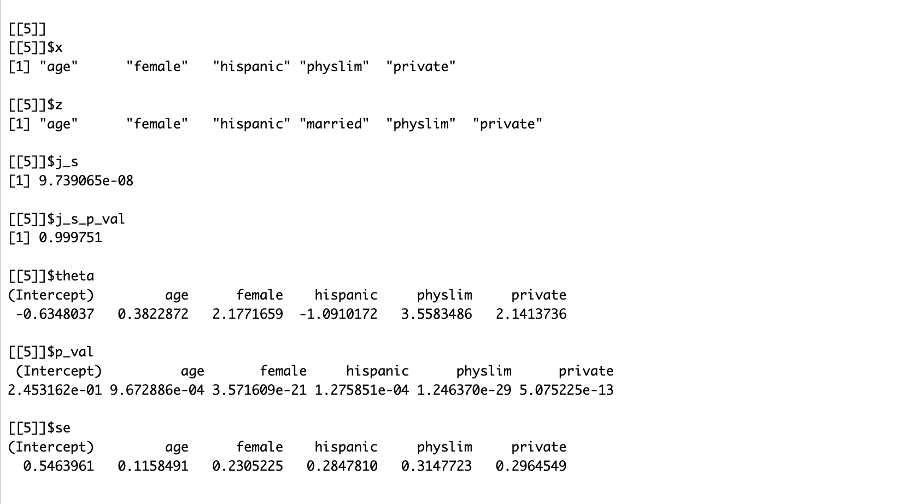
\includegraphics{5.png}



\newpage
\subsection{R code}
\begin{lstlisting}[language=R]
library(tidyverse)
library(rlang)
library(furrr)
library(momentfit)
library(tseries)

project<- read.csv("final_data.csv")

y= project$price_eur_m_whe

acf(y)  #autocorrelation
acf((y-mean(y))^2) #Heteroscedasticity 
adf.test(y) #stationary, Time series are stationary if they do not have trend or seasonal effects


gmm_2sls <- function(x, y, z) {
  x_hat <- z %*% solve(t(z) %*% z) %*% t(z) %*% x
  theta <- solve(t(x_hat) %*% x_hat) %*% t(x_hat) %*% y
  as.numeric(theta)
}


#check correlation and delete the variable has correlation greater than 0.8 (if you want to change another correlation, change 0.8 in the loop with other correlation you want)
del_mult_coll <- function(x) {
  x <- as.matrix(x)
  while (any(cor(x) > .8 & cor(x) < 1, na.rm = TRUE)) {
    i <- which(cor(x) > .8 & cor(x) < 1)[1] %% ncol(x)
    x <- x[, -i]
  }
  x
}

#define a set include all X and Z at first, if it have time variable, use -1, -2, and use time in first column and y in second column, if there has no time variable, only use ,1 and make sure y is in first colum
allxz <- del_mult_coll(select(project, -1, -2))

#The idea of the model is to first set up a total XZ dataset that we need, then bring in loop, which will calculate and find all the results that satisfy both the coefficient p-value and hesen test, and then store them in the allmodel set

gmm_model_select_n <- function(n, all_xz, y, data) {
  z_c <- combn(seq_len(ncol(all_xz)), n, NULL, FALSE)
  x_c <- list_c(map(seq_len(n - 1), \(i) {
    combn(seq_len(ncol(all_xz)), i, NULL, FALSE)
  }))
  all_comb <- expand_grid(seq_len(length(z_c)), seq_len(length(x_c)))
  plan(multisession, workers = 10) #Multi-threaded calls, run with as many cores as the computer needs, my test computer is a ten core cpu, so = 10
  all_mods <- array_branch(all_comb, 1) |>
    future_map(\(i) {
      z <- cbind(1, all_xz[, z_c[[i[1]]]])
      x <- cbind(1, all_xz[, x_c[[i[2]]]])
      theta <- try(gmm_2sls(x, y, z), silent = TRUE)
      if (inherits(theta, "try-error")) {
        j_s <- Inf
        j_s_p_val <- NULL
        p_val <- NULL
        se <- NULL
      } else {
        names(theta) <- c("(Intercept)", colnames(x)[-1])
        formula_x <- "price_eur_m_whe" |>
          paste(paste(colnames(all_xz)[x_c[[i[2]]]], collapse = " + "), sep = " ~ ") |>
          as.formula()
        formula_z <- paste("~", paste(colnames(all_xz)[z_c[[i[1]]]], collapse = " + ")) |>
          as.formula()
        test <- gmmFit(momentModel(formula_x, formula_z, data = data))
        p_val <- summary(test)@coef[, 4]
        se <- summary(test)@coef[, 2]
        j_s <- specTest(test)@test[, "Statistics"]
        j_s_p_val <- specTest(test)@test[, "pvalue"]
        if (sum(p_val > .05) > 1L) j_s <- Inf
      }
      list(
        x = colnames(x)[-1], z = colnames(z)[-1], j_s = j_s, j_s_p_val = j_s_p_val,
        theta = theta, p_val = p_val, se = se
      )
    })
  plan(sequential)
  all_mods
}

gmm_model_select <- function(all_xz, y, data) {
  all_mods <- list_c(map(
    seq_len(ncol(all_xz))[-1],
    gmm_model_select_n, all_xz, y, data
  ))
  j_ss <- map_dbl(all_mods, \(x) x$j_s)
  all_mods[order(j_ss)]
}

allmodel<-gmm_model_select(allxz,y,project)
allmodel[[1]]
with(allmodel[[1]], theta -1.96 * se) #CI, lower
with(allmodel[[1]], theta + 1.96 * se) #upper

\end{lstlisting}


\end{document}
